\documentclass{ximera}
\usepackage[colorlinks=true,linkcolor=blue]{hyperref}

\title{Setting up the repository}
\def\itemautorefname~#1\null{#1\null}
\begin{document}
\begin{abstract}
Instructions for setting up a repository containing course materials.
\end{abstract}
\maketitle

This tutorial is intended to help course instructors get a
\href{http://ximera.osu.edu}{\sf Ximera} 
course up and running. It guides the reader through the creation of a
\href{http://git-scm.com}{\sf git}
repository, the connection of the repository to
\href{http://github.com}{\tt github.com}
through a webhook, and the creation of an activity containing a 
simple exercise.

The instructions below assume that the reader will be
working on a computer running either Linux or OS X.
Similar instructions for Windows users will be composed
at a later stage, but the Linux instructions below will probably
be sufficient for Windows users with some familiarity with Unix commands.
While the reader could in principle avoid installing 
\href{http://texlive.org}{\LaTeX}\ and
\href{http://git-scm.com}{\sf git} these programs are necessary
to take full advantage of the features of the 
\href{http://ximera.osu.edu}{\sf Ximera} system.

\begin{warning} Currently {\em anyone} can
create a course on the webserver
\href{http://ximera.osu.edu}{\tt ximera.osu.edu}.
This is to say that if you follow the instructions below,
a new course that {\em you} control will appear on the web,
visable to all the world. It goes without saying therefore that
your course should not contain offensive or copyrighted
materials. However, in the future, it is quite likely that a
more robust course validation mechanism will be implemented.
\end{warning}

\subsection{Setting up a Ximera repository from scratch}
This section descdribes how to create a course from scratch.
Other possible ways to create
courses, such as forking existing courses, will
be discussed in \autoref{ForkClone}
\begin{enumerate}
\item\label{Mkdir} Create a directory for your course files
and change to that directory.
In this example, we will create a directory called
\verb!anExampleCourse!.
Open a terminal session and type the following commands.
\begin{center}
\begin{verbatim}
mkdir anExampleCourse
cd anExampleCourse 
\end{verbatim}
\end{center}

\item A \href{http://ximera.osu.edu}{\sf Ximera} 
course consists of a directory (the one
created above in this example)
containing a text file called \verb!course.xim!. 
In this tutorial we will create a simple
course consisting of only one activity.
Using any text editor, create and save a file named
\verb!course.xim! containing the text below.

\begin{verbatim}
---
name: An example course
description: This is a Ximera activity explaining how to get started with Ximera for course instructors.
---

theFirstActivity/theFirstActivity
\end{verbatim}
\begin{warning}
The content of the line beginning with \verb!name:!
specifies the title of your course exactly as it will appear on
\href{http://ximera.osu.edu/course}{\tt ximera.osu.edu/course}.
Without any further changes to \verb!course.xim!
your course will be listed as \verb!An example course!.
However, in order to distinguish your course from
other courses on
\href{http://ximera.osu.edu/course}{\tt ximera.osu.edu/course}
you should change the title to something unique
such as \verb!ISU Math 104!.
\end{warning}

\begin{remark}
In general the file \verb!course.xim! specifies course information
such as the name of the course, a description of the course,
and the names of all \LaTeX\ activity files 
comprising the course, in the order
they should be presented to students.
In addition to a name and a description,
the \verb!course.xim! file above specifies that 
there is one activity file \verb!theFirstActivity.tex!,
written without the extension \verb!.tex!,  
and located in a directory called \verb!theFirstActivity!.
We will create this file and directory in the following step.

Generally courses should contain more than one activity,
with each activity filename appearing in \verb!course.xim!
without its \verb!.tex! extension and
indented to reflect its position in the course hierarchy.
We recommend placing each
activity in a directory of the same name.
This facilitates
sharing activities among collaborators and makes reusing existing
activities easier.
%Later in this course, we will see examples of
%how to borrow existing activities from other courses
%rather than starting from scratch. 
We also recommend that the directory and the \LaTeX\ file have exactly
the same name as the title of the activity,
with all spaces removed and all words other than the first word
capitalized. So for example, if the title of the
activity were \verb!Plants native to Ohio!
the \LaTeX\ file \verb!plantsNativeToOhio.tex!
would be located in a directory called
\verb!plantsNativeToOhio!.
\end{remark}

\begin{warning}
The \verb!course.xim! file has particular formatting requirements.
\begin{enumerate}
\item The name of the file must be exactly \verb!course.xim!
\item The \verb!---!'s encapsulating the name on line~2
and the description on line~3
are required, as is the blank line following the second \verb!---!.
\item All the entries between the \verb!---!'s
must be written as single lines. 
In other words, the only newlines permitted are those
at the end of lines~2 and 3.
\end{enumerate}
\end{warning}

\item In your terminal create a new directory
in the \verb!anExampleCourse! directory
called \verb!theFirstActivity!. The \verb!theFirstActivity!
directory should contain a file called \verb!theFirstActivity.tex!.
This can be accomplished by
executing the commands below.
\begin{verbatim}
mkdir theFirstActivity 
cd theFirstActivity 
touch theFirstActivity.tex
\end{verbatim}

\item\label{FirstExercise}
Using your text editor, open \verb!theFirstActivity.tex!
and paste in the following text. Then save the file.
\begin{verbatim}
\documentclass{ximera}
\title{The First Activity}
\begin{document}
\begin{abstract}
This activity deals with \verb!Ximera! activities.
\end{abstract}
\maketitle
\end{document}
\end{verbatim}

\begin{remark}
An activity should be composed as a regular
\LaTeX\ file in the document class \verb!ximera!.
It should contain the title of the activity and an abstract.
These will both appear on the course website in the navigation area,
so the abstract should be short.
At this stage your activity contains
a title and an abstract, but is otherwise blank.
\end{remark}

\item\label{GithubCreate}
Log into your \href{http://github.com}{\tt github.com}
account and create a repository with the name
\verb!anExampleCourse!
by clicking the \verb!+! by your account name, as shown
in the image below.

\begin{image}
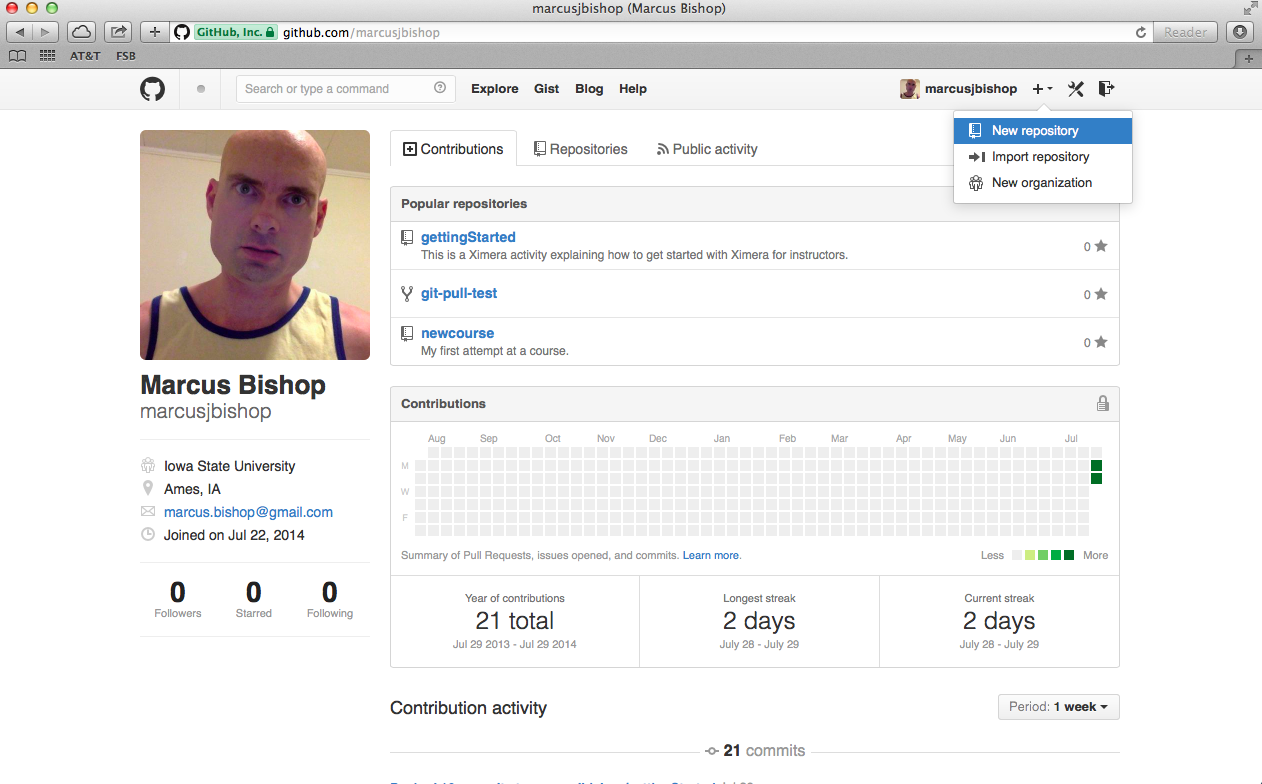
\includegraphics[scale=.3]{RepoInit.png}
\end{image}

After selecting \verb!New repository! from the dropdown menu, a new
page appears with a field named \verb!Repository name!. Enter
\verb!anExampleCourse! into this field and
accept all the default settings by pressing the green
\verb!Create Repository! button.
\begin{image}
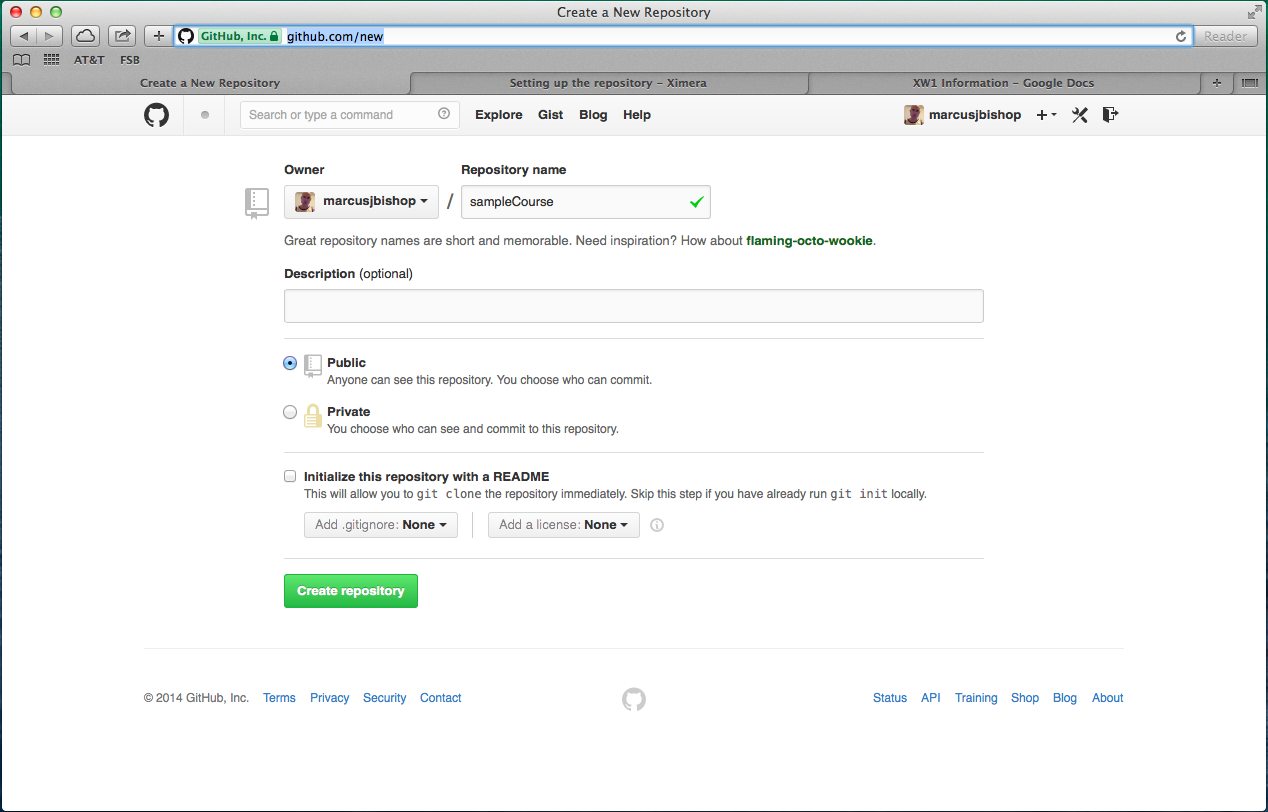
\includegraphics[scale=.3]{CreateRepo.png}
\end{image}
\href{http://github.com}{\tt github.com}
will respond by printing additional commands similar to
those shown below.
\begin{verbatim}
touch README.md
git init
git add README.md
git commit -m "first commit"
git remote add origin https://github.com/marcusjbishop/anExampleCourse.git
git push -u origin master
\end{verbatim}
Before executing these commands, return
to your terminal and ensure that your current directory is
\verb!anExampleCourse!. 
If your current directory is \verb!theFirstActivity!
from the previous step you can change to its parent directory by typing
\begin{verbatim}
cd ..
\end{verbatim}
Now execute the commands returned by
\href{http://github.com}{\tt github.com}.

\begin{remark}
Note that your username appears in the fifth line
of these commands in place of \verb!marcusjbishop!.
Note also the \verb!s! in \verb!https!.
These commands initialize the repository on \href{http://github.com}{\tt github.com}
and create an empty file named \verb!README.md!
in the \verb!anExampleCourse! directory.
\end{remark}

\item Execute the following command, still in the
\verb!anExampleCourse! directory.
\begin{verbatim}
git add .
\end{verbatim}
\begin{remark}
Note that the command above contains a dot at the end.
This command adds the newly created directory
\verb!theFirstActivity! and the files
\verb!theFirstActivity/theFirstActivity.tex!
and \verb!course.xim! to your repository.
In general a \verb!git add! command must be executed
every time a new file or directory is created.
\end{remark}

\item This step is optional. Type a
description of your course in the file
\verb!README.md!.

\begin{remark}
The content of \verb!README.md! will appear only on
\href{http://github.com}{\tt github.com}.
This file is meant to provide a description of your project
to other developers.
\end{remark}

\item Click the \verb!Settings! button on your
\href{http://github.com}{\tt github.com} repository page
and then on \verb!Webhooks & Services!.
Now click the \verb!Add webhook! button.
Type \verb!http://ximera.osu.edu/github!
into the \verb!Payload URL! field and
\verb!8mi0tsrje9n3asPu86XC198G1XSdZj!
into the \verb!Secret! field.
\begin{image}
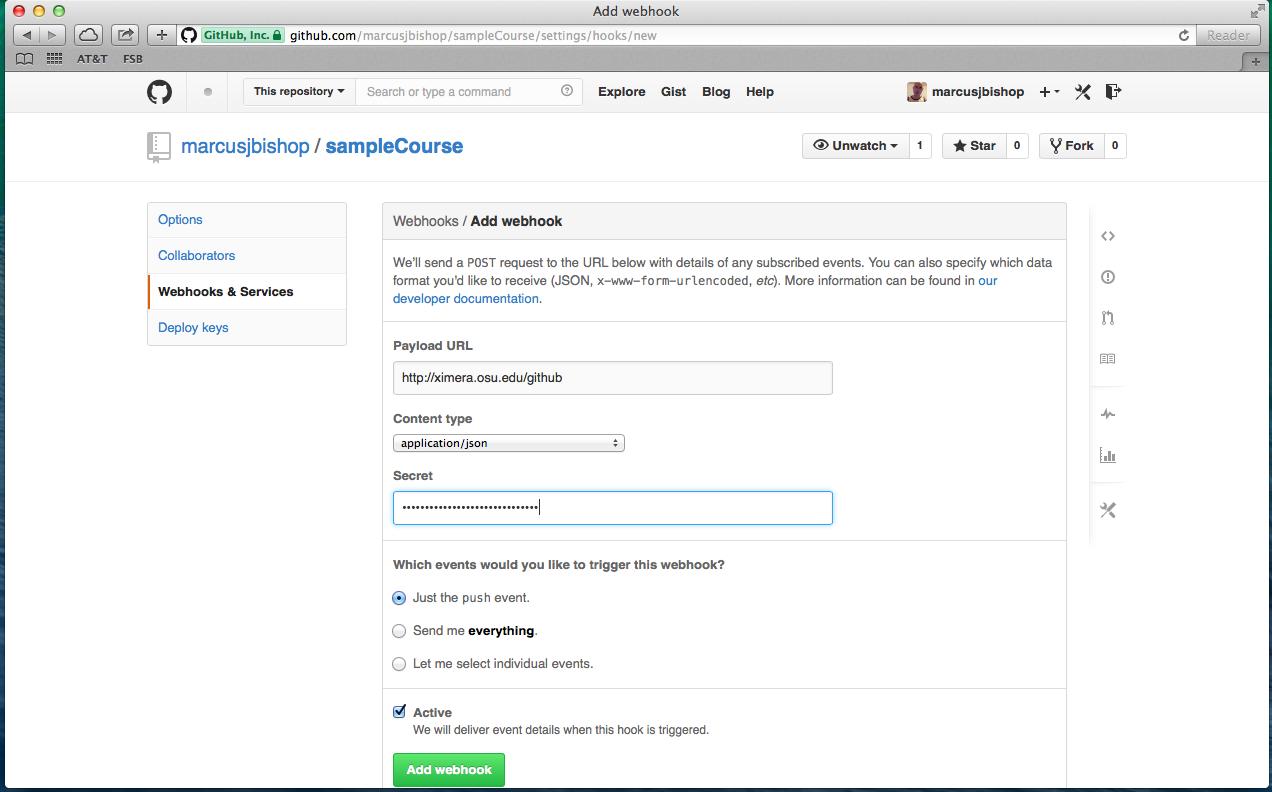
\includegraphics[scale=.3]{Webhook.png}
\end{image}
Finally push the green \verb!Add webhook! button at the bottom
of the window.

\item
In order to have your course served by
\href{http://ximera.osu.edu/course}{\tt ximera.osu.edu/course}
you need to \verb!push! your repository.
However, since \textsf{git} will not allow a \verb!push!
if you haven't made any changes to the repository,
this is a good point to add some further content
in the form of a simple exercise.
Update the file \verb!theFirstActivity.tex! 
you created above so that it looks like the following. 

\begin{verbatim}
\documentclass{ximera}
\title{The First Activity}
\begin{document}
\begin{abstract}
This activity deals with \verb!Ximera! activities.
\end{abstract}
\maketitle
This activity is about creative work.
\begin{exercise}
  Choose the best place to work on mathematics.
  \begin{multipleChoice}
    \choice{At the library}
    \choice[correct]{At the caf\'e}
    \choice{In your office}
  \end{multipleChoice}
\end{exercise}
\end{document}
\end{verbatim}
\begin{remark}
The edits above insert
a multiple-choice question into the \verb!theFirstActivity!
activity. See the {\em Question and answer types}
activity later in this tutorial
for more information on creating exercises.
\end{remark}

\item Change to the directory \verb!anExampleCourse!
and execute the following commands.
\begin{verbatim}
git commit -am "Added an exercise"
git push
\end{verbatim}
If everything went well, you should find your course listed at 
\href{http://ximera.osu.edu/course}{\tt ximera.osu.edu/course}.
If not, see the {\em Troubleshooting} activity in this tutorial
or send your questions to
\href{mailto:ximera@math.osu.edu}{\tt ximera@math.osu.edu}.
\begin{remark} The commands above inform 
\href{http://git-scm.com}{\sf git} that
changes have been made to your repository and 
communicates them to
\href{http://github.com}{\tt github.com}
which in turn communicates them to
\href{http://ximera.osu.edu}{\tt ximera.osu.edu}.
You should execute similar commands whenever you
change files in your repository.
\end{remark}
\end{enumerate}

\subsection{Other ways to set up a Ximera repository}
There are other ways to create a
\href{http://ximera.osu.edu}{\sf Ximera} course.
One possibility is to begin by creating the repository on
\href{http://github.com}{\tt github.com}
as in step~\autoref{GithubCreate} above.
Then instead of executing the commands
that follow to initialize the local copy of the repository,
you could {\em clone} the copy on 
\href{http://github.com}{\tt github.com} using a
\verb!git clone! command.
Alternately you could {\em fork} an existing repository,
either your own or someone else's.
See the \href{http://git-scm.com}{{\sf git} manual}
for more information about the \verb!clone! and \verb!fork! commands.
Both possibilities above obviate step \autoref{Mkdir} since cloning
or forking a \href{http://git-scm.com}{\sf git} repository
creates a local directory and initializes
it as a \href{http://git-scm.com}{\sf git} repository.

From here you can create 
\href{http://ximera.osu.edu}{\sf Ximera} 
activities as in step~\autoref{FirstExercise}.
You should issue a \verb!git add! command after creating
a new file or directory and a \verb!git commit!
command followed by a \verb!git push! command
periodically to transmit your most recent changes to
\href{http://github.com}{\tt github.com}.
You should also add the name of your activity file without
its \verb!.tex! extension to the file \verb!course.xim!
it the position relative to other activities where
you want the activity to appear.
Observe however that once the filename
appears in \verb!course.xim! the corresponing activity will appear
to students. It might therefore be preferable
to {\em not} add the filename to \verb!course.xim!
until the activity is ready for students.
During the editing phase you still view
the activity by processing it with \LaTeX\ and inspecting
the resulting PDF file, which might be helpful 
in any case for finding and correcting mistakes.

Still another possitility is to create and edit {\em all} files
and directories directly on the
\href{http://github.com}{\tt github.com} web site.
In this way you could produce an entire
\href{http://ximera.osu.edu}{\sf Ximera} 
course {\em without} a local copy of the repository.
This would have the advantage of not requiring the
instructor to install the
\href{http://git-scm.com}{\sf git} or
\href{http://texlive.org}{\LaTeX}\ software
or to learn any of the
\href{http://git-scm.com}{\sf git} or Unix
commands above. This could be useful when working temporarily on
someone else's computer, for example.

\end{document}
